\documentclass{article}
\usepackage{graphicx}
\usepackage{caption}
\usepackage{subcaption}
\usepackage{mwe}
\usepackage{subfig}
\usepackage{listings}

\begin{document}

\title{Medical Imaging - Homework 2}
\author{Paniz Karbasi}

\maketitle

\section{Problem 1}

In this problem, first the three images related to the three different sinograms have been illustrated in Figures~\ref{sino1}-~\ref{sino3}. Based on these images, the sinogram that is created by additive Gaussian noise (Figure~\ref{sino2}) has some amount of noise in the background of the image that is visible to the eye, but the noise is very small. On the other hand, the image that is created by adding the Gaussian noise to the original image and then constructing the sinogram (Figure~\ref{sino3}), has visibly distorted signals, because when we perform the radon transform, at each angle, we are adding the signal and the noise together, therefore the final sinogram is distorted significantly.



When reconstructing images with FBP and ART algorithms, the images related to the third sinogram in Figure~\ref{sino3}, contain more noise, in comparison with the images reconstructed with the sinogram in Figure~\ref{sino2}. The reason is because of the fact that the measurements vector or sinogram, contains much more noise in the case of Figure~\ref{sino3} than Figure~\ref{sino2}, thus, the noise is then added back to the reconstructed image. In the case of the sinogram with additive noise (Figure~\ref{sino2}), the reconstructed images are closer to the images reconstructed with the true sinogram because the sinogram with additive Gaussian noise contains a small amount of noise that is added back to the images.


\newpage
\begin{figure}[h]
\centering
  
\includegraphics{sino1.png}
  \caption{True Sinogram}\label{sino1}
\end{figure}

\newpage
\begin{figure}[h]
  
\includegraphics[width=\linewidth]{sino2.png}
  \caption{Sinogram with Additive Gaussian Noise}\label{sino2}
\end{figure}

\newpage
\begin{figure}[h]
  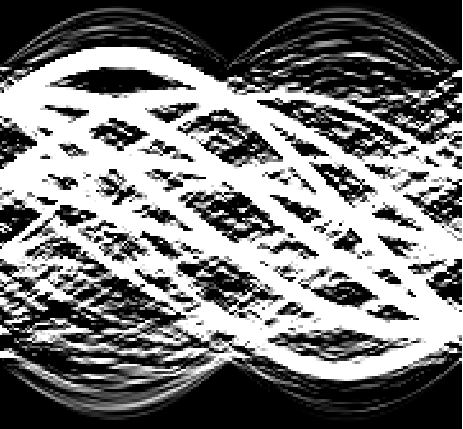
\includegraphics[width=\linewidth]{sino3.png}
  \caption{Sinogram of the True image with Additive Gaussian Noise}\label{sino3}
\end{figure}

\newpage
\begin{figure}[h]
\centering
  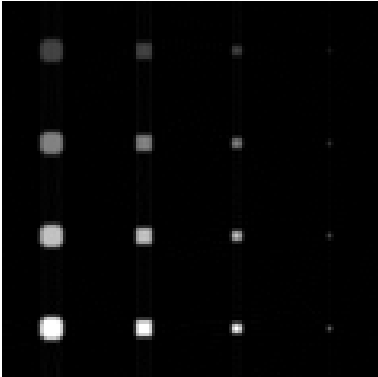
\includegraphics{FBP1.png}
  \caption{FBP Image of True Sinogram}\label{fbp1}
\end{figure}

\newpage
\begin{figure}[h]
  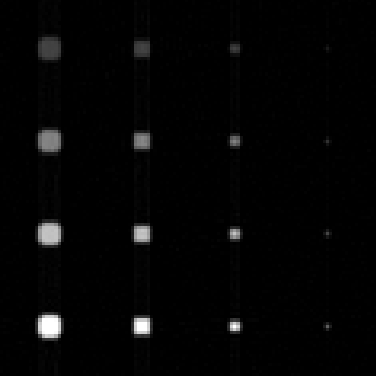
\includegraphics[width=\linewidth]{FBP2.png}
  \caption{FBP Image of Sinogram with Additive Gaussian Noise}\label{fbp2}
\end{figure}

\newpage
\begin{figure}[h]
  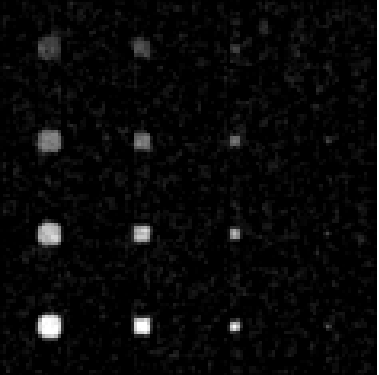
\includegraphics[width=\linewidth]{FBP3.png}
  \caption{FBP Image of Sinogram of the True image with Additive Gaussian Noise}\label{fbp3}
\end{figure}


\newpage
\begin{figure}[h]
\centering
  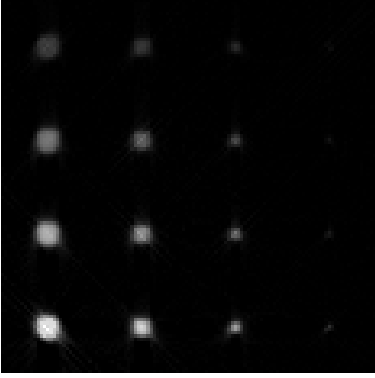
\includegraphics{ART1.png}
  \caption{ART Image of True Sinogram}\label{fbp1}
\end{figure}

\newpage
\begin{figure}[h]
  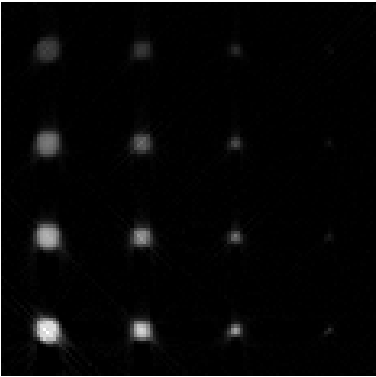
\includegraphics[width=\linewidth]{ART2.png}
  \caption{ART Image of Sinogram with Additive Gaussian Noise}\label{fbp2}
\end{figure}


\newpage
\begin{figure}[h]
  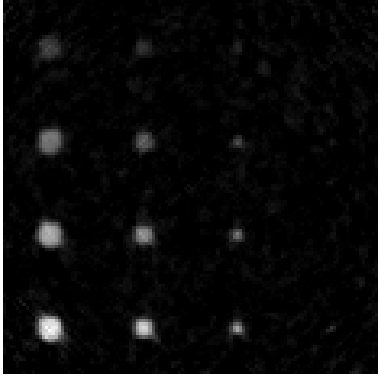
\includegraphics[width=\linewidth]{ART3.png}
  \caption{ART Image of Sinogram of the True image with Additive Gaussian Noise}\label{fbp3}
\end{figure}

\newpage
\subsection{Matlab Code}
\lstinputlisting{Reconstruction_demo.m}
\lstinputlisting{FBP.m}
\lstinputlisting{ART.m}

\newpage

\section{Problem 2}
The image 12 image slices reconstructed with the FBP are illustrated in the following pages. The way these images have been reconstructed is based on the fact that we need 12 sinograms. Therefore, for each height, the sinogram has been formed and then the image has been reconstructed with the FBP.

\begin{figure}[t!] % "[t!]" placement specifier just for this example
\begin{subfigure}{0.45\textwidth}

\includegraphics[width=\linewidth]{s_01.png}
\caption{Slice 1} \label{fig:a}
\end{subfigure}\hspace*{\fill}
\begin{subfigure}{0.45\textwidth}

\includegraphics[width=\linewidth]{s_02.png}
\caption{Slice 2} \label{fig:b}
\end{subfigure}

\medskip
\begin{subfigure}{0.45\textwidth}
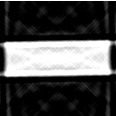
\includegraphics[width=\linewidth]{s_03.png}
\caption{Slice 3} \label{fig:c}
\end{subfigure}\hspace*{\fill}
\begin{subfigure}{0.45\textwidth}
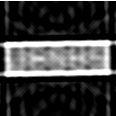
\includegraphics[width=\linewidth]{s_04.png}
\caption{Slice 4} \label{fig:d}
\end{subfigure}

\medskip
\begin{subfigure}{0.45\textwidth}
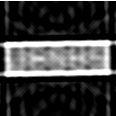
\includegraphics[width=\linewidth]{s_05.png}
\caption{Slice 5} \label{fig:e}
\end{subfigure}\hspace*{\fill}
\begin{subfigure}{0.45\textwidth}
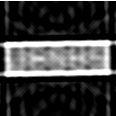
\includegraphics[width=\linewidth]{s_06.png}
\caption{Slice 6} \label{fig:f}
\end{subfigure}

\caption{FBP Images of Slices 1 through 6} \label{fig:1}
\end{figure}

\begin{figure}[t!] % "[t!]" placement specifier just for this example
\begin{subfigure}{0.45\textwidth}
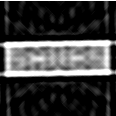
\includegraphics[width=\linewidth]{s_07.png}
\caption{Slice 7} \label{fig:a}
\end{subfigure}\hspace*{\fill}
\begin{subfigure}{0.45\textwidth}
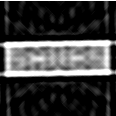
\includegraphics[width=\linewidth]{s_08.png}
\caption{Slice 8} \label{fig:b}
\end{subfigure}

\medskip
\begin{subfigure}{0.45\textwidth}
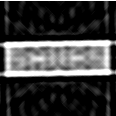
\includegraphics[width=\linewidth]{s_09.png}
\caption{Slice 9} \label{fig:c}
\end{subfigure}\hspace*{\fill}
\begin{subfigure}{0.45\textwidth}
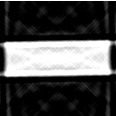
\includegraphics[width=\linewidth]{s_10.png}
\caption{Slice 10} \label{fig:d}
\end{subfigure}

\medskip
\begin{subfigure}{0.45\textwidth}

\includegraphics[width=\linewidth]{s_11.png}
\caption{Slice 11} \label{fig:e}
\end{subfigure}\hspace*{\fill}
\begin{subfigure}{0.45\textwidth}

\includegraphics[width=\linewidth]{s_12.png}
\caption{Slice 12} \label{fig:f}
\end{subfigure}

\caption{FBP Images of Slices 7 through 12} \label{fig:1}
\end{figure}



\subsection{Matlab Code}
\lstinputlisting{Reconstruction_Unknown_Object.m}


\end{document}